\documentclass[tikz,border=4pt]{standalone}
\usepackage[T1]{fontenc}
\usepackage{lmodern}
\renewcommand{\familydefault}{\sfdefault}
\usetikzlibrary{shapes.geometric,positioning,arrows.meta,calc,fit,backgrounds,decorations.pathreplacing}
\tikzset{
  node distance=6mm,
  every node/.style={font=\footnotesize,align=center,execute at begin node={\hyphenpenalty=10000\relax}},
  base/.style={draw=gray!60,fill=gray!12,minimum height=7mm,inner sep=2pt},
  term/.style={base,rounded corners=3.5mm,text width=30mm},
  proc/.style={base,text width=32mm},
  err/.style={base,text width=30mm,fill=gray!22},
  io/.style={base,trapezium,trapezium left angle=72,trapezium right angle=108,trapezium stretches=true,text width=28mm},
  dec/.style={base,diamond,aspect=2.4,text width=27mm,inner sep=0pt},
  % predefined process: a call to another procedure
  sub/.style={proc,inner xsep=3mm,path picture={
    \draw[gray!60] ([xshift=1.5mm]path picture bounding box.north west)--([xshift=1.5mm]path picture bounding box.south west)
                   ([xshift=-1.5mm]path picture bounding box.north east)--([xshift=-1.5mm]path picture bounding box.south east);}},
  go/.style={-{Stealth[length=2mm]},draw=gray!55!black},
  lab/.style={font=\scriptsize,fill=white,inner sep=1pt},
  frame/.style={draw=gray!60,dashed,rounded corners=2mm,inner sep=3mm},
  % memory diagrams
  cell/.style={draw=gray!60,fill=gray!12,minimum height=7mm,inner sep=1pt,font=\scriptsize},
  hot/.style={cell,fill=gray!35},
  note/.style={font=\scriptsize,text=gray!30!black},
}

\begin{document}
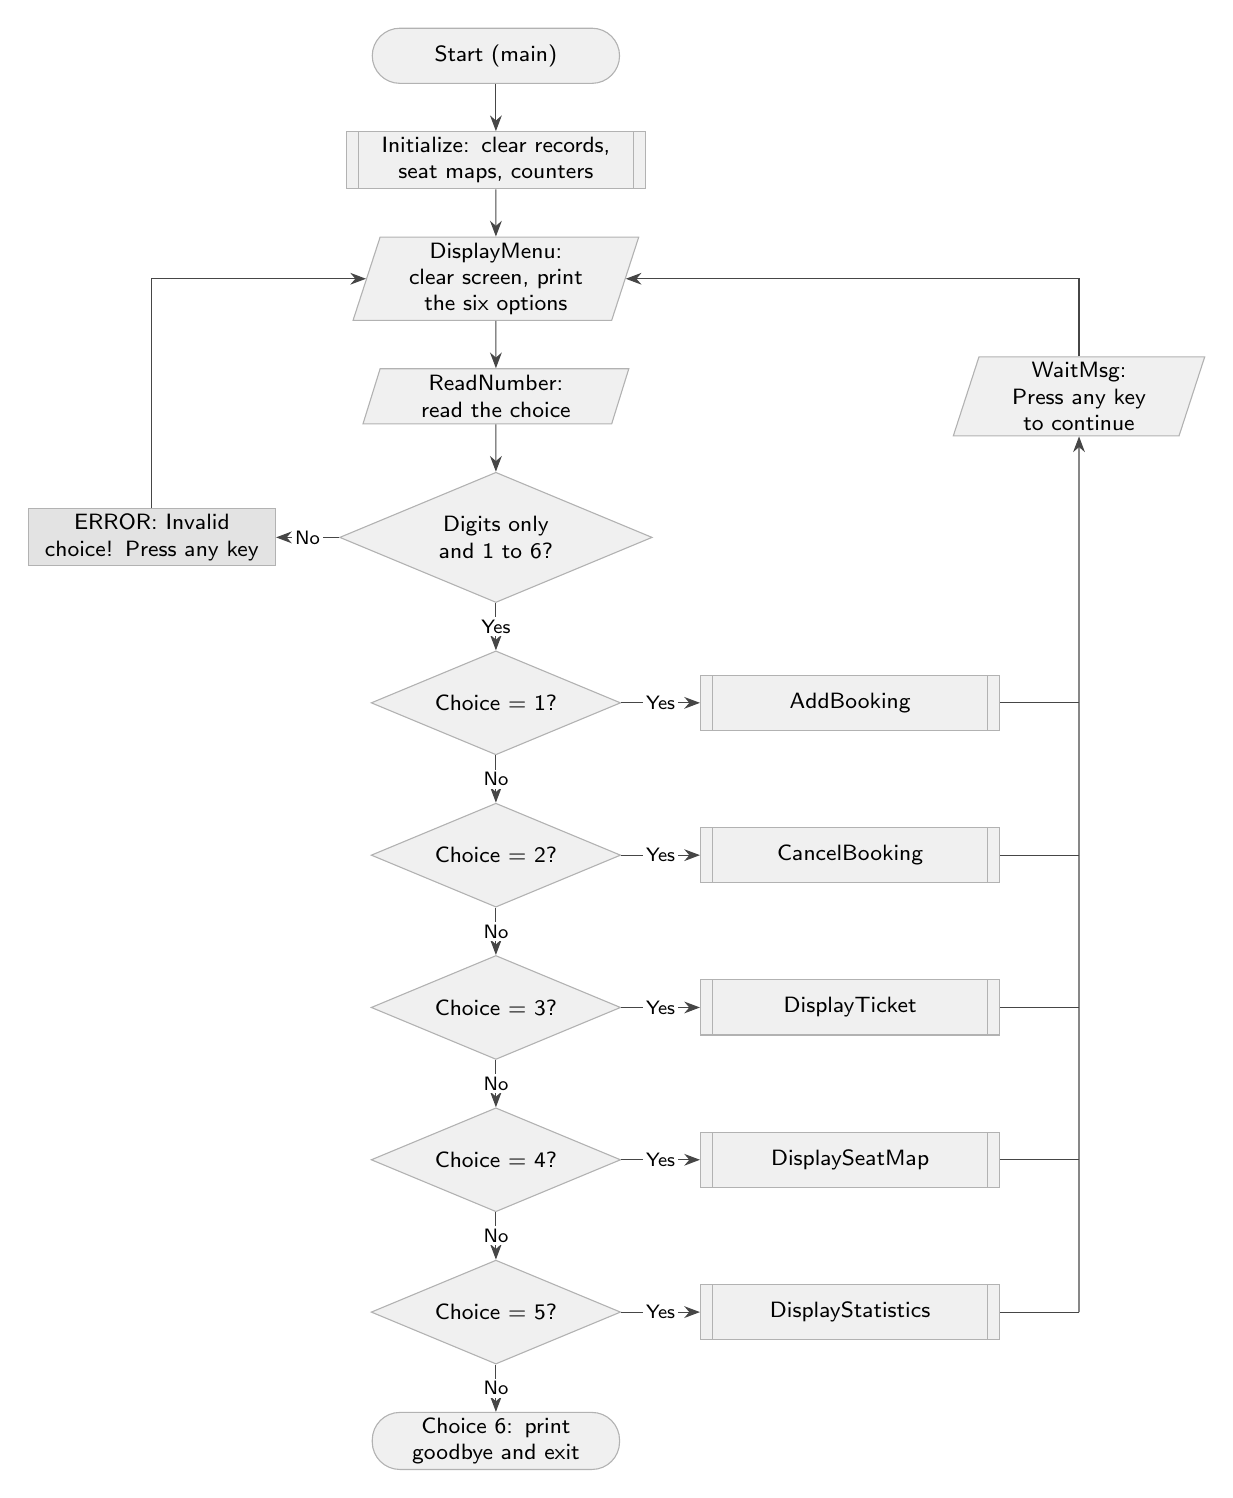
\begin{tikzpicture}
\node[term] (s) {Start (main)};
\node[sub,below=of s] (init) {Initialize: clear records, seat maps, counters};
\node[io,below=of init] (menu) {DisplayMenu: clear screen, print the six options};
\node[io,below=of menu] (rd) {ReadNumber: read the choice};
\node[dec,below=of rd] (v) {Digits only and 1 to 6?};
\node[err,left=8mm of v] (e) {ERROR: Invalid choice! Press any key};
\node[dec,below=of v] (c1) {Choice = 1?};
\node[dec,below=of c1] (c2) {Choice = 2?};
\node[dec,below=of c2] (c3) {Choice = 3?};
\node[dec,below=of c3] (c4) {Choice = 4?};
\node[dec,below=of c4] (c5) {Choice = 5?};
\node[term,below=of c5] (x) {Choice 6: print goodbye and exit};
\node[sub,right=10mm of c1] (a1) {AddBooking};
\node[sub,right=10mm of c2] (a2) {CancelBooking};
\node[sub,right=10mm of c3] (a3) {DisplayTicket};
\node[sub,right=10mm of c4] (a4) {DisplaySeatMap};
\node[sub,right=10mm of c5] (a5) {DisplayStatistics};
\coordinate (bus) at ($(a1.east)+(10mm,0)$);
\node[io,text width=24mm] (w) at (bus |- rd) {WaitMsg: Press any key to continue};
\draw[go] (s)--(init);
\draw[go] (init)--(menu);
\draw[go] (menu)--(rd);
\draw[go] (rd)--(v);
\draw[go] (v)--node[lab]{No}(e);
\draw[go] (e.north)|-(menu.west);
\draw[go] (v)--node[lab]{Yes}(c1);
\foreach \i/\j in {1/2,2/3,3/4,4/5}{\draw[go] (c\i)--node[lab]{No}(c\j);}
\draw[go] (c5)--node[lab]{No}(x);
\foreach \i in {1,...,5}{
  \draw[go] (c\i)--node[lab]{Yes}(a\i);
  \draw[draw=gray!55!black] (a\i.east)--(a\i.east -| bus);}
\draw[go] (a5.east -| bus)--(w.south);
\draw[go] (w.north)|-(menu.east);
\end{tikzpicture}
\end{document}
